% Options for packages loaded elsewhere
\PassOptionsToPackage{unicode}{hyperref}
\PassOptionsToPackage{hyphens}{url}
%
\documentclass[
]{article}
\usepackage{amsmath,amssymb}
\usepackage{iftex}
\ifPDFTeX
  \usepackage[T1]{fontenc}
  \usepackage[utf8]{inputenc}
  \usepackage{textcomp} % provide euro and other symbols
\else % if luatex or xetex
  \usepackage{unicode-math} % this also loads fontspec
  \defaultfontfeatures{Scale=MatchLowercase}
  \defaultfontfeatures[\rmfamily]{Ligatures=TeX,Scale=1}
\fi
\usepackage{lmodern}
\ifPDFTeX\else
  % xetex/luatex font selection
\fi
% Use upquote if available, for straight quotes in verbatim environments
\IfFileExists{upquote.sty}{\usepackage{upquote}}{}
\IfFileExists{microtype.sty}{% use microtype if available
  \usepackage[]{microtype}
  \UseMicrotypeSet[protrusion]{basicmath} % disable protrusion for tt fonts
}{}
\makeatletter
\@ifundefined{KOMAClassName}{% if non-KOMA class
  \IfFileExists{parskip.sty}{%
    \usepackage{parskip}
  }{% else
    \setlength{\parindent}{0pt}
    \setlength{\parskip}{6pt plus 2pt minus 1pt}}
}{% if KOMA class
  \KOMAoptions{parskip=half}}
\makeatother
\usepackage{xcolor}
\usepackage[margin=1in]{geometry}
\usepackage{color}
\usepackage{fancyvrb}
\newcommand{\VerbBar}{|}
\newcommand{\VERB}{\Verb[commandchars=\\\{\}]}
\DefineVerbatimEnvironment{Highlighting}{Verbatim}{commandchars=\\\{\}}
% Add ',fontsize=\small' for more characters per line
\usepackage{framed}
\definecolor{shadecolor}{RGB}{248,248,248}
\newenvironment{Shaded}{\begin{snugshade}}{\end{snugshade}}
\newcommand{\AlertTok}[1]{\textcolor[rgb]{0.94,0.16,0.16}{#1}}
\newcommand{\AnnotationTok}[1]{\textcolor[rgb]{0.56,0.35,0.01}{\textbf{\textit{#1}}}}
\newcommand{\AttributeTok}[1]{\textcolor[rgb]{0.13,0.29,0.53}{#1}}
\newcommand{\BaseNTok}[1]{\textcolor[rgb]{0.00,0.00,0.81}{#1}}
\newcommand{\BuiltInTok}[1]{#1}
\newcommand{\CharTok}[1]{\textcolor[rgb]{0.31,0.60,0.02}{#1}}
\newcommand{\CommentTok}[1]{\textcolor[rgb]{0.56,0.35,0.01}{\textit{#1}}}
\newcommand{\CommentVarTok}[1]{\textcolor[rgb]{0.56,0.35,0.01}{\textbf{\textit{#1}}}}
\newcommand{\ConstantTok}[1]{\textcolor[rgb]{0.56,0.35,0.01}{#1}}
\newcommand{\ControlFlowTok}[1]{\textcolor[rgb]{0.13,0.29,0.53}{\textbf{#1}}}
\newcommand{\DataTypeTok}[1]{\textcolor[rgb]{0.13,0.29,0.53}{#1}}
\newcommand{\DecValTok}[1]{\textcolor[rgb]{0.00,0.00,0.81}{#1}}
\newcommand{\DocumentationTok}[1]{\textcolor[rgb]{0.56,0.35,0.01}{\textbf{\textit{#1}}}}
\newcommand{\ErrorTok}[1]{\textcolor[rgb]{0.64,0.00,0.00}{\textbf{#1}}}
\newcommand{\ExtensionTok}[1]{#1}
\newcommand{\FloatTok}[1]{\textcolor[rgb]{0.00,0.00,0.81}{#1}}
\newcommand{\FunctionTok}[1]{\textcolor[rgb]{0.13,0.29,0.53}{\textbf{#1}}}
\newcommand{\ImportTok}[1]{#1}
\newcommand{\InformationTok}[1]{\textcolor[rgb]{0.56,0.35,0.01}{\textbf{\textit{#1}}}}
\newcommand{\KeywordTok}[1]{\textcolor[rgb]{0.13,0.29,0.53}{\textbf{#1}}}
\newcommand{\NormalTok}[1]{#1}
\newcommand{\OperatorTok}[1]{\textcolor[rgb]{0.81,0.36,0.00}{\textbf{#1}}}
\newcommand{\OtherTok}[1]{\textcolor[rgb]{0.56,0.35,0.01}{#1}}
\newcommand{\PreprocessorTok}[1]{\textcolor[rgb]{0.56,0.35,0.01}{\textit{#1}}}
\newcommand{\RegionMarkerTok}[1]{#1}
\newcommand{\SpecialCharTok}[1]{\textcolor[rgb]{0.81,0.36,0.00}{\textbf{#1}}}
\newcommand{\SpecialStringTok}[1]{\textcolor[rgb]{0.31,0.60,0.02}{#1}}
\newcommand{\StringTok}[1]{\textcolor[rgb]{0.31,0.60,0.02}{#1}}
\newcommand{\VariableTok}[1]{\textcolor[rgb]{0.00,0.00,0.00}{#1}}
\newcommand{\VerbatimStringTok}[1]{\textcolor[rgb]{0.31,0.60,0.02}{#1}}
\newcommand{\WarningTok}[1]{\textcolor[rgb]{0.56,0.35,0.01}{\textbf{\textit{#1}}}}
\usepackage{graphicx}
\makeatletter
\def\maxwidth{\ifdim\Gin@nat@width>\linewidth\linewidth\else\Gin@nat@width\fi}
\def\maxheight{\ifdim\Gin@nat@height>\textheight\textheight\else\Gin@nat@height\fi}
\makeatother
% Scale images if necessary, so that they will not overflow the page
% margins by default, and it is still possible to overwrite the defaults
% using explicit options in \includegraphics[width, height, ...]{}
\setkeys{Gin}{width=\maxwidth,height=\maxheight,keepaspectratio}
% Set default figure placement to htbp
\makeatletter
\def\fps@figure{htbp}
\makeatother
\setlength{\emergencystretch}{3em} % prevent overfull lines
\providecommand{\tightlist}{%
  \setlength{\itemsep}{0pt}\setlength{\parskip}{0pt}}
\setcounter{secnumdepth}{-\maxdimen} % remove section numbering
\ifLuaTeX
  \usepackage{selnolig}  % disable illegal ligatures
\fi
\usepackage{bookmark}
\IfFileExists{xurl.sty}{\usepackage{xurl}}{} % add URL line breaks if available
\urlstyle{same}
\hypersetup{
  pdftitle={Public Transport Winterbottlenecks},
  pdfauthor={Leonard, Stefan, Pascal},
  hidelinks,
  pdfcreator={LaTeX via pandoc}}

\title{Public Transport Winterbottlenecks}
\usepackage{etoolbox}
\makeatletter
\providecommand{\subtitle}[1]{% add subtitle to \maketitle
  \apptocmd{\@title}{\par {\large #1 \par}}{}{}
}
\makeatother
\subtitle{\href{https://github.com/paACode/publictransport_winterbottlenecks_palest}{Public
GitHub Repository}}
\author{Leonard, Stefan, Pascal}
\date{17.05.2025}

\begin{document}
\maketitle

{
\setcounter{tocdepth}{3}
\tableofcontents
}
\section{Introduction}\label{introduction}

Zentralbahn, a regional railway company, identified a pressing need to
improve the overall performance of its train operations. In response,
the company initiated a comprehensive, data-driven investigation aimed
at uncovering operational inefficiencies and ensuring long-term service
reliability.

As part of this initiative, Zentralbahn engaged an external data science
consultant to analyze publicly available OpenTransportData. The
consultant's initial findings revealed a noticeable performance
bottleneck in November 2024, likely linked to seasonal, winter-related
disruptions.

Although Zentralbahn already had an internal hypothesis regarding the
cause, the company is committed to an open, evidence-based approach and
is seeking independent confirmation and fresh insights. To broaden the
analytical perspective, Zentralbahn partnered with the Hochschule Luzern
(HSLU) to carry out a dedicated project using operational data from
November 2024.

\section{Project Goals}\label{project-goals}

\textbf{1. Identifying Root Causes of Performance Bottlenecks}

The primary objective is to analyze train operations during
\textbf{November 2024} to:

\begin{itemize}
\tightlist
\item
  Validate Zentralbahn's internal assumptions about winter-related
  disruptions,
\item
  Identify underlying patterns or unexpected factors contributing to
  performance bottlenecks,
\item
  Provide data-driven recommendations for improving punctuality and
  operational efficiency on affected lines.
\end{itemize}

\textbf{2. Improving Data Quality Through Predictive Modeling }

A secondary goal is to address known data quality issues in
Zentralbahn's internal datasets. Specifically, several records contain
\textbf{missing or incorrect train station entries}. HSLU is tasked
with:

\begin{itemize}
\tightlist
\item
  Investigating the \textbf{November 2024 dataset}, which is considered
  consistent and reliable,
\item
  Exploring the potential to \textbf{predict or classify missing train
  station values} using available variables such as timestamps, route
  IDs, or event sequences,
\item
  Developing a methodology that could later be applied to
  \textbf{recover and correct corrupted historical datasets}.
\end{itemize}

\section{Report Structure}\label{report-structure}

The following chapters present different approaches to modeling. The
analysis begins with a general approach, using an initial artificial
neural network (ANN) without extensive knowledge of the data. It then
progresses toward more granular and detailed models. In the final
chapter, the insights gained throughout the analysis are consolidated
and integrated into a comprehensive model.

\section{A First Look: Artificial Neural
Network}\label{a-first-look-artificial-neural-network}

This chapter investigates the predictability of train cancellations
without performing prior exploratory data analysis (EDA). It serves as
an initial attempt to understand the underlying data. More detailed
analyses using simpler and more interpretable models will follow in
subsequent chapters.

An artificial neural network (ANN) enables the construction of a
predictive model without requiring extensive knowledge of the data
structure. It can provide early indications of whether the data contains
a meaningful signal.

Therefore, the approach directly attempts to predict whether a train is
cancelled, using all available variables, except those that explicitly
reveal cancellation status. These are:

\begin{itemize}
\tightlist
\item
  \texttt{AN\_PROGNOSE} and \texttt{AB\_PROGNOSE}: Always \texttt{NA}
  when a train is cancelled
\item
  \texttt{AN\_PROGNOSE\_STATUS} and \texttt{AB\_PROGNOSE\_STATUS}:
  Always \texttt{"UNBEKANNT"} when cancelled
\item
  All derived columns such as:

  \begin{itemize}
  \tightlist
  \item
    \texttt{ABFAHRTDELAY\_sec}, \texttt{ABFAHRTDELAY\_min}
  \item
    \texttt{ANKUNFTDELAY\_sec}, \texttt{ANKUNFTDELAY\_min}
  \item
    \texttt{RUSH\_HOUR}, \texttt{TAGESZEIT}, \texttt{DELAY\_CATEGORY}
  \item
    \texttt{ZIEL}, \texttt{START}
  \end{itemize}
\end{itemize}

These variables are excluded to avoid data leakage.

\subsection{Data Preparation}\label{data-preparation}

As a first step, the distribution of the response variable is examined.
An initial analysis indicates that 21\% of the trains in the dataset are
cancelled. This was taken into account during data preparation. For the
ANN to work, the following steps were performed:

\begin{enumerate}
\def\labelenumi{\arabic{enumi}.}
\tightlist
\item
  Convert character and logical variables to factors\\
\item
  Remove factors with fewer than two levels (contain no information)\\
\item
  Use only factor variables to keep the ANN simple\\
\item
  Drop time columns because they include a large number of levels\\
\item
  Perform one-hot encoding\\
\item
  Stratify train and test data\\
\item
  Downsample train data to ensure an equal number of cancelled and
  uncancelled trains
\end{enumerate}

\subsection{Building the Network}\label{building-the-network}

Building the Network included a lot of trial and error. Because for many
configurations the model did not converge. In the end 3 predictors could
be found which lead to quite good prediction:

\begin{itemize}
\tightlist
\item
  BETRIEBSTAG
\item
  LINIEN\_TEXT
\item
  HALTESTELLEN\_NAME
\end{itemize}

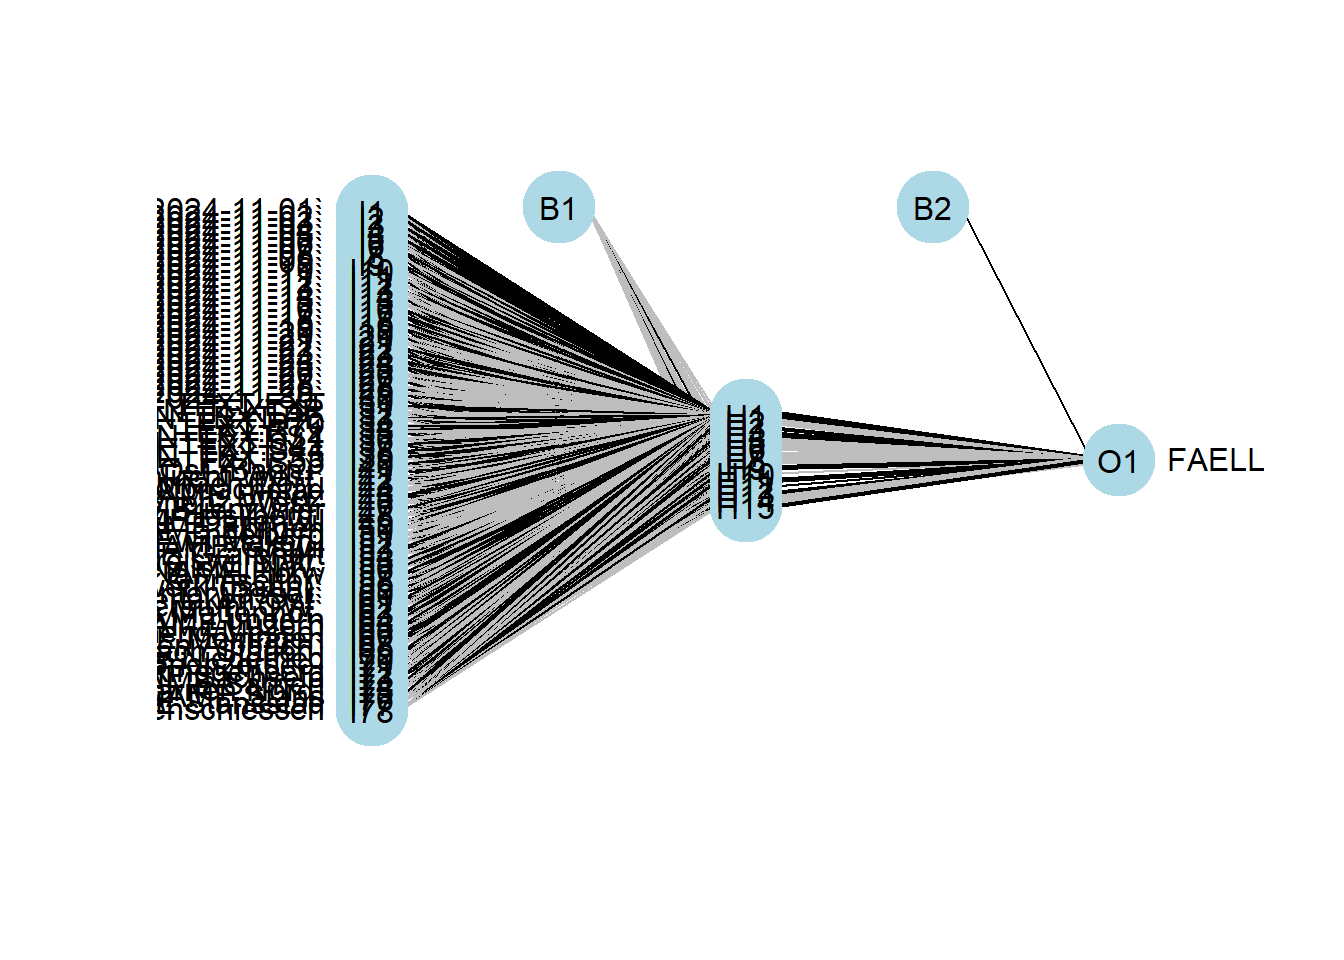
\includegraphics{final_documentation_files/figure-latex/Plot NET-1.pdf}

\subsection{Results}\label{results}

The model successfully predicts train cancellations using only three
categorical predictors: \textbf{BETRIEBSTAG}, \textbf{LINIEN\_TEXT}, and
\textbf{HALTESTELLEN\_NAME}. Despite the test data containing 80\%
uncancelled and 20\% cancelled trains, the model performs well thanks to
stratification and downsampling during training.

Given this class imbalance, accuracy alone is not the most informative
metric. Instead, specificity provides a more meaningful evaluation of
the model's ability to correctly identify cancelled trains.
Encouragingly, the model attains a specificity of 95.43\%, indicating
reliable detection of cancellations within the cancelled train
instances.

These findings highlight that these predictors are valuable features and
warrant further exploration through more detailed modeling and analysis.

\begin{verbatim}
       true
pred    FALSE  TRUE
  FALSE 14291   172
  TRUE    199  3591
\end{verbatim}

\begin{verbatim}
Confusion Matrix and Statistics

          Reference
Prediction FALSE  TRUE
     FALSE 14291   172
     TRUE    199  3591
                                          
               Accuracy : 0.9797          
                 95% CI : (0.9775, 0.9817)
    No Information Rate : 0.7938          
    P-Value [Acc > NIR] : <2e-16          
                                          
                  Kappa : 0.9381          
                                          
 Mcnemar's Test P-Value : 0.1771          
                                          
            Sensitivity : 0.9863          
            Specificity : 0.9543          
         Pos Pred Value : 0.9881          
         Neg Pred Value : 0.9475          
             Prevalence : 0.7938          
         Detection Rate : 0.7829          
   Detection Prevalence : 0.7924          
      Balanced Accuracy : 0.9703          
                                          
       'Positive' Class : FALSE           
                                          
\end{verbatim}

\section{Generalised Additive Model}\label{generalised-additive-model}

In this project, we apply Generalized Additive Models (GAMs) to analyze
the effects of various predictors on train delays, specifically focusing
on the response variables ANKUNFTDELAY\_min (arrival delay in minutes)
and ABFAHRTDELAY\_min (departure delay in minutes). Due to the limited
availability of continuous variables in our dataset these two delay
metrics will be the response variables we will focus on. A key subset of
our predictors is related to weather conditions. However, because the ZB
railway line spans multiple climatic regions, comparing weather-related
predictors across all stations introduces variability that may obscure
meaningful patterns. To address this, we restrict our analysis to a
subset of stations located within the Lucerne region, where the climate
is more uniform.

R assumes for GAM models the Gaussian family for the response variables.
Therefore, let's have a look if the response variables ANKUNFTDELAY\_min
and ABFAHRTDELAY\_min are Gaussian distributed.

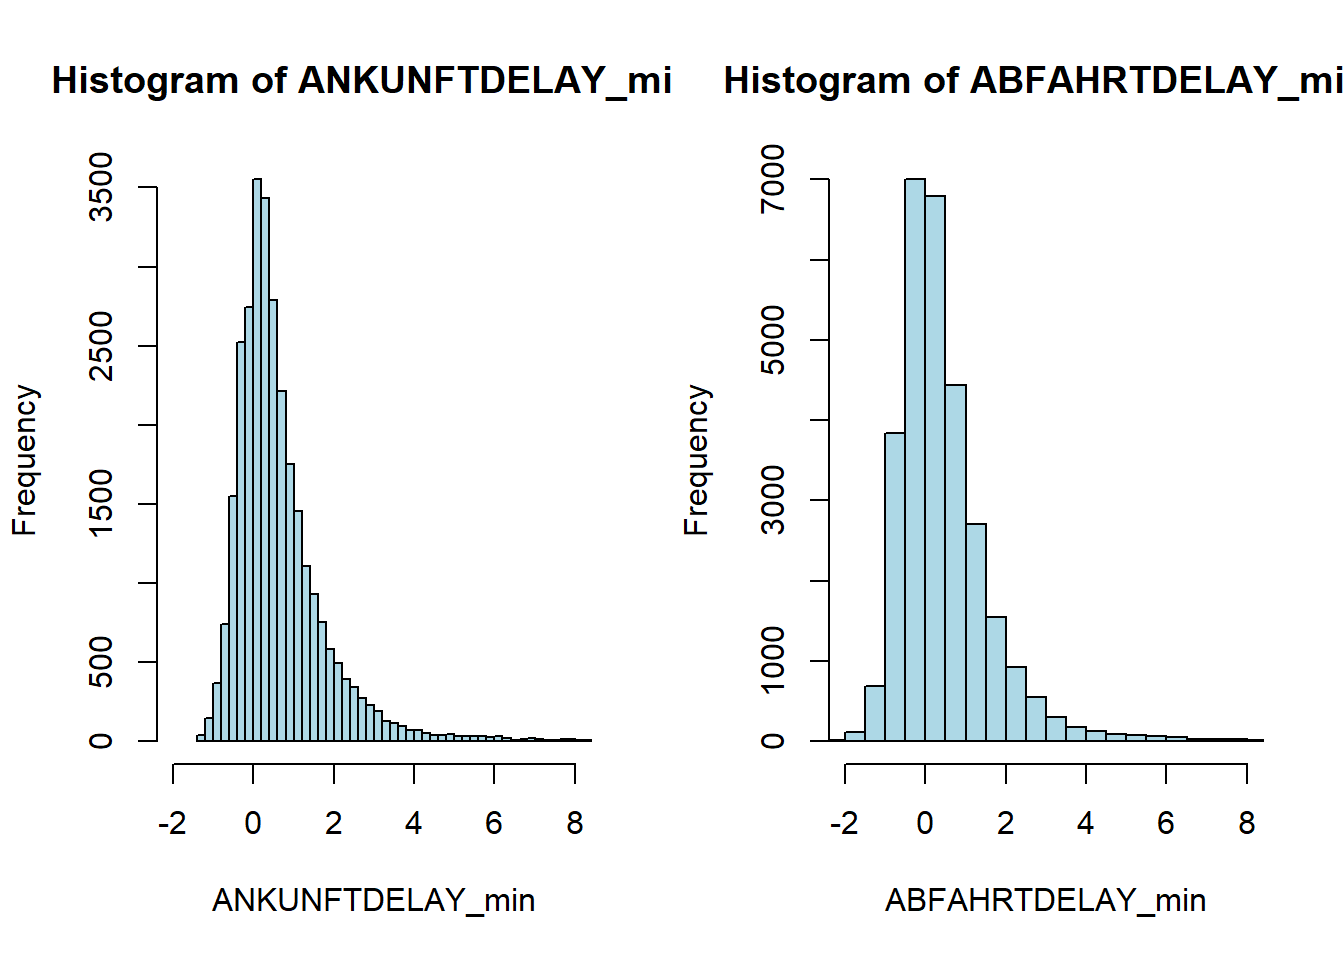
\includegraphics{final_documentation_files/figure-latex/first-histogram-1.pdf}

We see that both response variables are not normally distributed. In
real-world train operations, early arrivals or departures are relatively
uncommon compared to delays. Moreover, the distribution indicates that
longer delays occur less frequently than shorter ones, reflecting
typical delay patterns observed in Swiss public transportation. For this
reason, we restrict our dataset for the GAM analysis to observations
with delays between -2 and +4 minutes, aiming to ensure a distribution
that more closely approximates the Gaussian assumption required by the
model.

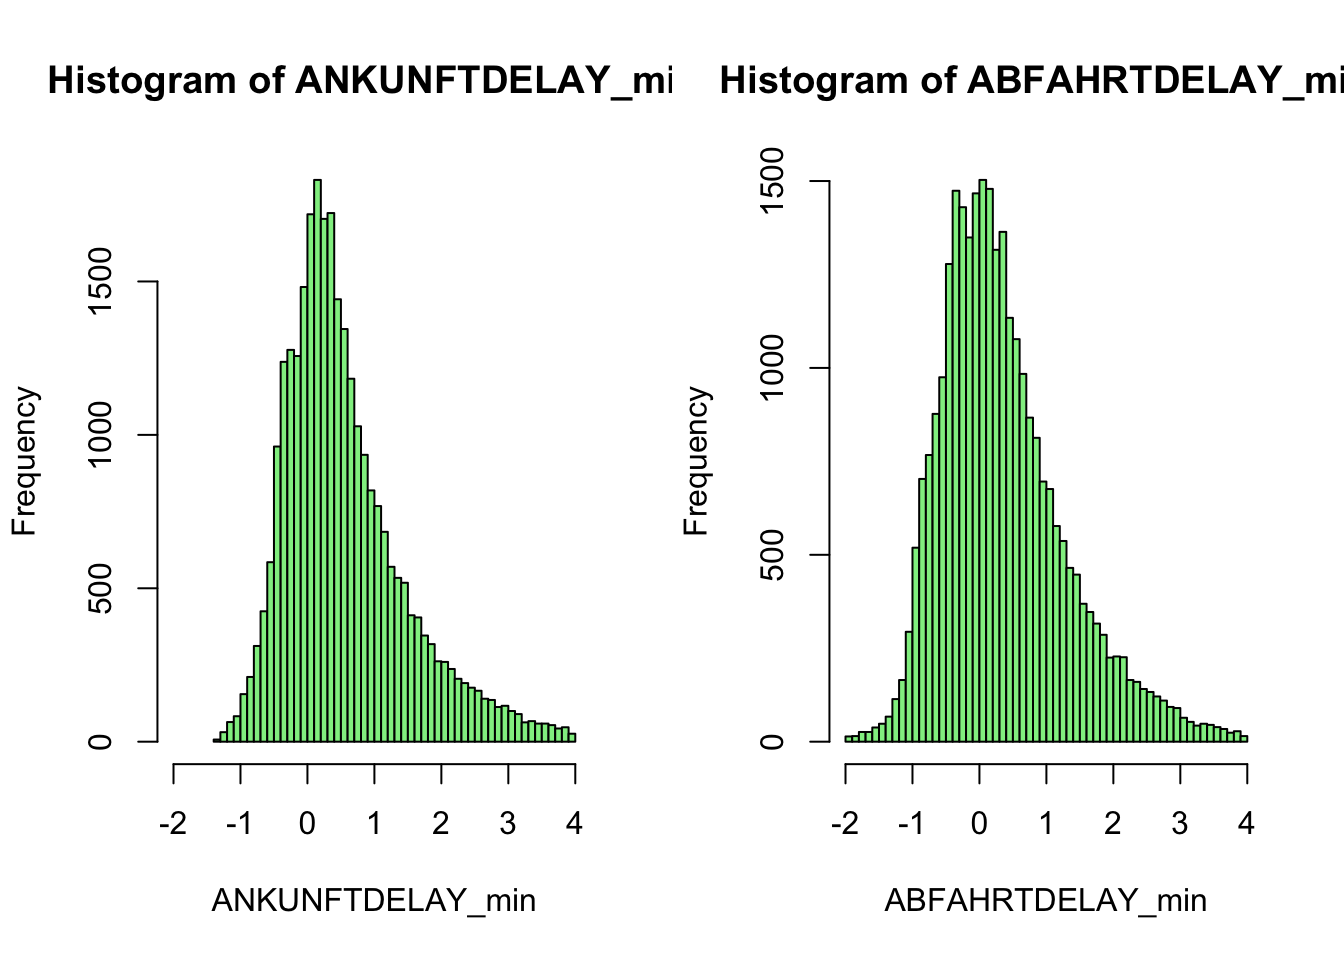
\includegraphics{final_documentation_files/figure-latex/second-histogram-1.pdf}

The histogram indicates an approximately normal distribution. Therefore,
the dataset is now suitable for fitting with Generalized Additive Models
(GAMs).

\begin{verbatim}

Family: gaussian 
Link function: identity 

Formula:
ANKUNFTDELAY_min ~ s(w_temp_avg_c_Luzern)

Parametric coefficients:
            Estimate Std. Error t value Pr(>|t|)    
(Intercept)  0.56586    0.00519     109   <2e-16 ***
---
Signif. codes:  0 '***' 0.001 '**' 0.01 '*' 0.05 '.' 0.1 ' ' 1

Approximate significance of smooth terms:
                         edf Ref.df   F p-value    
s(w_temp_avg_c_Luzern) 8.881  8.995 122  <2e-16 ***
---
Signif. codes:  0 '***' 0.001 '**' 0.01 '*' 0.05 '.' 0.1 ' ' 1

R-sq.(adj) =  0.0364   Deviance explained = 3.67%
GCV = 0.78087  Scale est. = 0.7806    n = 28984
\end{verbatim}

The p-value associated with the smooth term is close to zero, providing
strong evidence that the average temperature in Lucerne has a
statistically significant effect on arrival delays. The estimated
effective degrees of freedom (edf ≈ 9) suggest a moderately complex,
non-linear relationship. However, the adjusted R-squared value of 0.036
and the explained deviance of only 3.67\% indicate that the model
captures only a small portion of the variation in arrival delays. Thus,
while the effect is significant, temperature alone does not explain much
of the delay variability.

\begin{verbatim}

Family: gaussian 
Link function: identity 

Formula:
ABFAHRTDELAY_min ~ TAGESZEIT + LINIEN_TEXT + s(w_temp_avg_c_Luzern) + 
    s(w_precip_mm_Luzern)

Parametric coefficients:
                    Estimate Std. Error t value Pr(>|t|)    
(Intercept)          1.24747    0.33220   3.755 0.000174 ***
TAGESZEITMittag     -0.30000    0.01880 -15.961  < 2e-16 ***
TAGESZEITNachmittag -0.16098    0.01854  -8.682  < 2e-16 ***
TAGESZEITNacht      -0.30080    0.01631 -18.441  < 2e-16 ***
TAGESZEITVormittag  -0.11592    0.01655  -7.002 2.57e-12 ***
LINIEN_TEXTIR       -0.22497    0.33290  -0.676 0.499183    
LINIEN_TEXTPE       -2.32029    0.93772  -2.474 0.013352 *  
LINIEN_TEXTS4       -0.83845    0.33198  -2.526 0.011555 *  
LINIEN_TEXTS41      -1.35328    0.33415  -4.050 5.14e-05 ***
LINIEN_TEXTS44      -1.04235    0.33382  -3.122 0.001795 ** 
LINIEN_TEXTS5       -0.50933    0.33200  -1.534 0.125008    
LINIEN_TEXTS55      -1.95525    0.33936  -5.762 8.41e-09 ***
---
Signif. codes:  0 '***' 0.001 '**' 0.01 '*' 0.05 '.' 0.1 ' ' 1

Approximate significance of smooth terms:
                         edf Ref.df     F p-value    
s(w_temp_avg_c_Luzern) 9.000  9.000 79.03  <2e-16 ***
s(w_precip_mm_Luzern)  8.319  8.591 59.29  <2e-16 ***
---
Signif. codes:  0 '***' 0.001 '**' 0.01 '*' 0.05 '.' 0.1 ' ' 1

R-sq.(adj) =  0.119   Deviance explained = 11.9%
GCV = 0.76993  Scale est. = 0.76915   n = 28984
\end{verbatim}

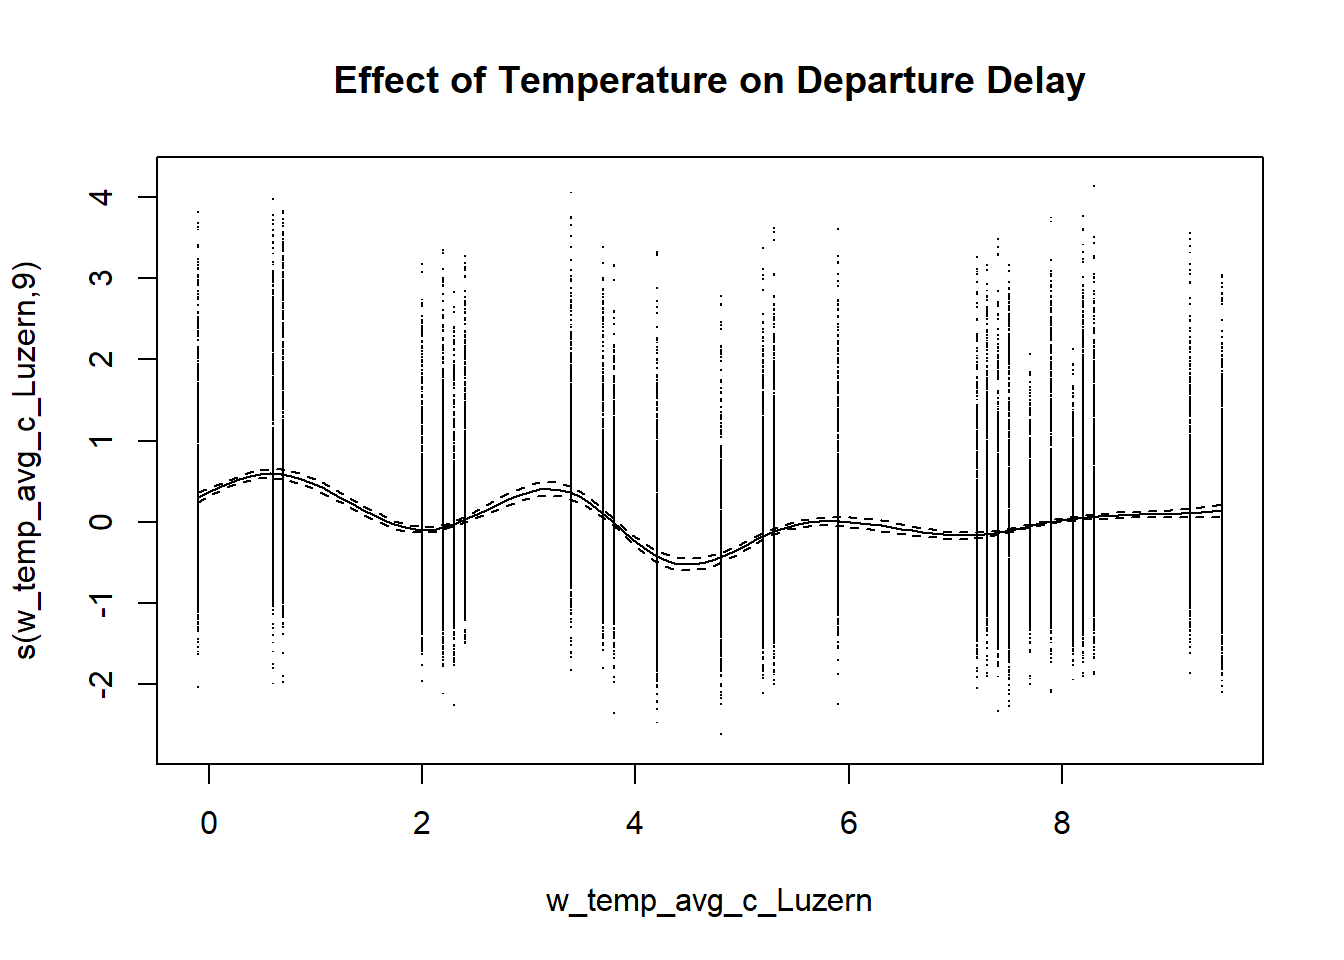
\includegraphics{final_documentation_files/figure-latex/gam-temp-precip-tageszeit-linien_text-1.pdf}
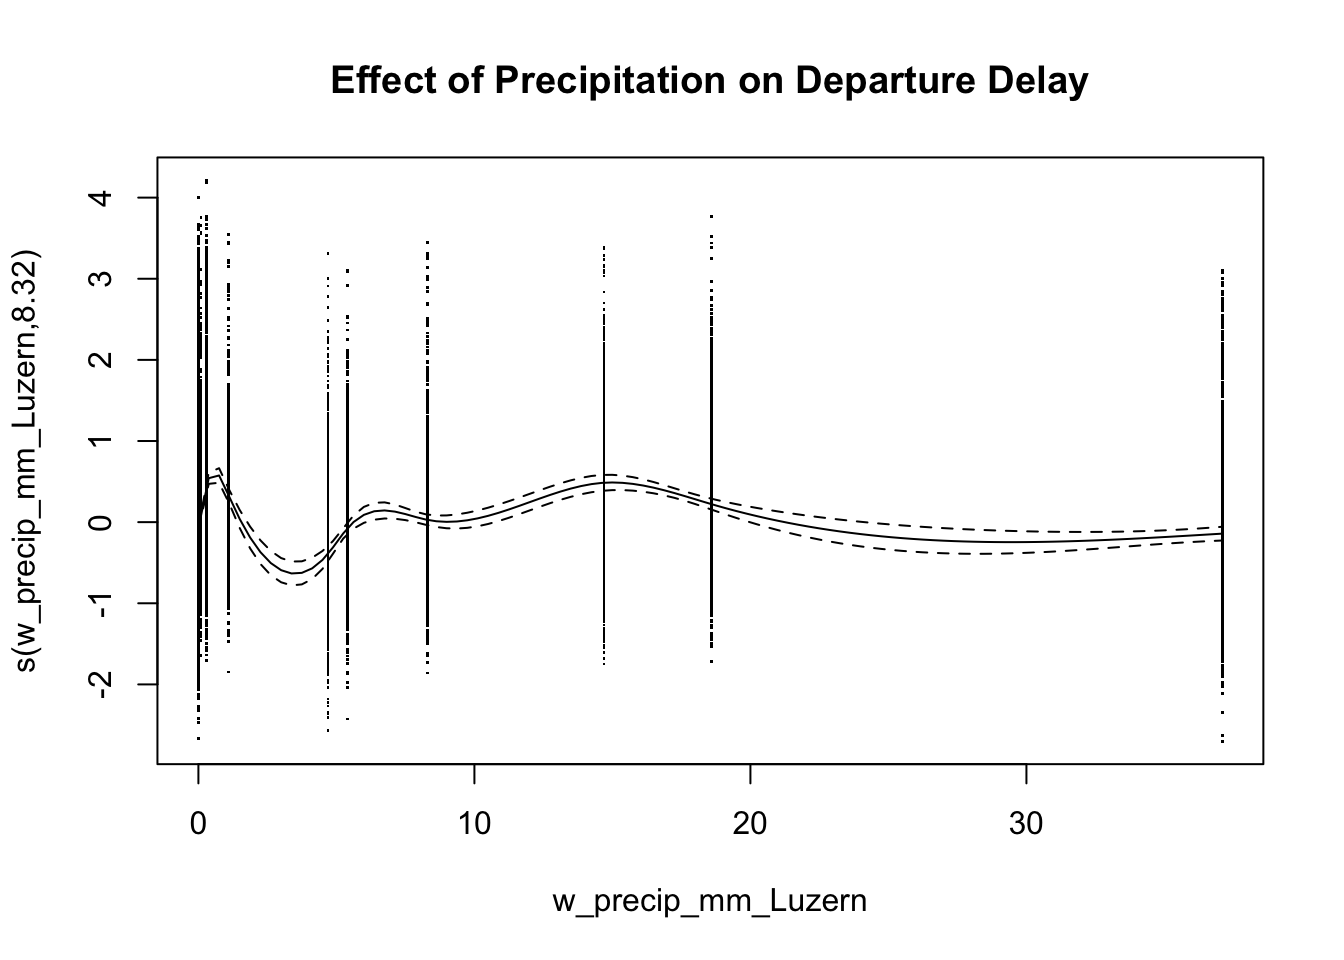
\includegraphics{final_documentation_files/figure-latex/gam-temp-precip-tageszeit-linien_text-2.pdf}

Interpretation of Parametric Coefficients:

The reference levels for the categorical predictors are evening for
TAGESZEIT and EXT for LINIEN\_TEXT. Under these baseline conditions
(evening, 0°C, and 0 mm precipitation), the EXT line of ZB in the
Lucerne region has an average departure delay of approximately 1.25
minutes.

The effect of time of day is not substantial; compared to the evening,
trains experience during the other times of the day on average 0.12 -
0.3 minutes less delays.

Regarding train lines, the IR line shows a reduction of 0.22 minutes
compared to EXT, although this difference is not statistically
significant (p = 0.5). In contrast, the PE line exhibits the largest
reduction, with trains experiencing on average 2.32 minutes less delay
than EXT, a difference that is statistically significant. Likewise, the
S4, S41, S44, and S55 lines show significantly reduced delays compared
to EXT, with reductions of 0.84, 1.35, 1.04, and 1.96 minutes,
respectively. The S5 line's difference (0.51 minutes less) is not
statistically significant.

Interpretation of the Smooth Terms:

The smooth term for average temperature has an estimated effective
degrees of freedom (edf) of approximately 9, indicating a moderately
complex non-linear relationship with departure delay. We have strong
evidence that it is not 0 with a p-value \textless{} 0.05. The
corresponding plot reveals that temperatures between 0 and 6°C have a
stronger effect on departure delay, whereas between roughly 6--7°C and
8--10°C the effect is minimal.

Similarly, the smooth term for average precipitation
(w\_precip\_mm\_Luzern) has an edf of about 8.32, suggesting a
moderately complex non-linear relationship. We have strong evidence that
it is not 0 with a p-value \textless{} 0.05.

The precipitation plot shows a clear non-linear relationship between
precipitation and departure delays. There is a strong effect at lower
precipitation levels (up to approximately 20 mm), after which the curve
flattens between around 22 mm and 50 mm, indicating a reduced impact on
delays. One possible explanation for this flattening is that higher
precipitation levels may coincide with times of reduced train
activity---such as during the night---when fewer departures occur,
thereby minimizing the observed effect on overall delays. Additionally,
since the dataset only covers November 2024, it is possible that there
were relatively few instances of heavy precipitation during this period
in the Lucerne region, which may limit the model's ability to capture
stronger effects at higher precipitation levels.

Overall model performance:

The adjusted R² value of 0.119 means that the model explains around
11.9\% of the variation in departure delays. This suggests that the
predictors included in the model have a measurable effect on delays, but
a large part of the variation (around 88\%) is still not accounted for.
This can be considered as not unusual in real-world transportation data,
where many factors that influence delays---such as technical problems,
temporary disruptions, staffing issues or operational decisions---are
not included in the dataset. While the model successfully identifies
several statistically significant predictors, it also shows that more
variables or more complex modeling approaches might be needed to better
capture all the factors that contribute to departure delays.

Conclusion:

GAM analysis revealed that weather factors significantly impact train
delays in the Lucerne region, aligning with the project's goal to
understand winter-related disruptions in November. However, the models
capture only a small portion of the variability, suggesting further
investigation is needed to fully explain performance bottlenecks.

\section{Generalised Linear Model with family set to
Binomial}\label{generalised-linear-model-with-family-set-to-binomial}

To further investigate the factors influencing train delays on the
Zentralbahn network, a Generalized Linear Model (GLM) with a binomial
family is applied. This model aims to predict the likelihood of a train
being delayed based on key operational variables, including train line
and rush hour status. By classifying delays as a binary outcome, the
analysis provides deeper insights into line-specific vulnerabilities and
the broader operational challenges faced during peak travel times. This
contributes to the project's overarching goal of identifying root causes
of performance bottlenecks and improving punctuality through data-driven
strategies.

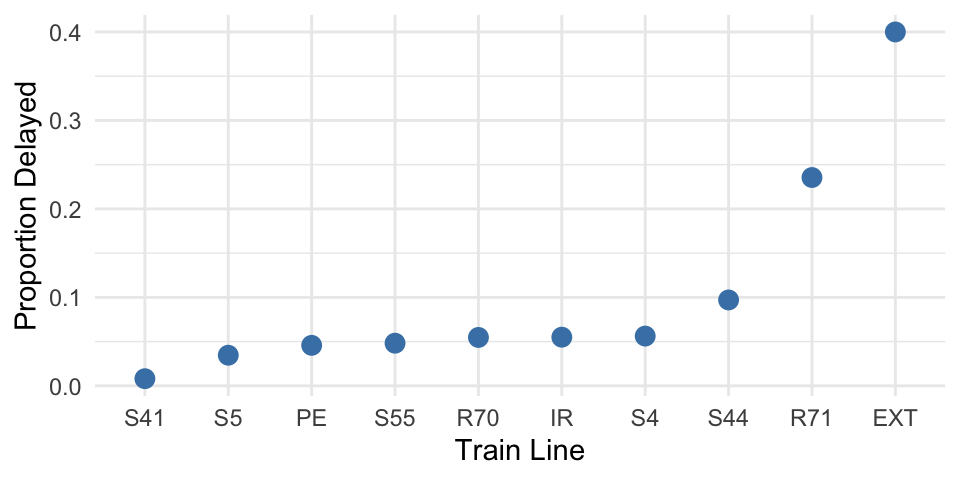
\includegraphics{final_documentation_files/figure-latex/first-plotting-1.pdf}

In this plot, we can see that the EXT line has the highest proportion of
delayed trains, with approximately 40\% of its services experiencing
delays. The line with the second highest delay rate is the R71, where
around 24\% of trains are delayed. On the other end of the spectrum, the
S41 line shows the lowest delay rate, with only about 1\% of its trains
being delayed.

To predict whether a train is delayed, we use a binomial GLM with
Train\_Delayed as the binary response variable and LINIEN\_TEXT (train
line) as the predictor. This model estimates how the probability of
delay varies across different train lines.

\begin{verbatim}

Call:
glm(formula = Train_Delayed ~ LINIEN_TEXT, family = "binomial", 
    data = zb_final_binominal)

Coefficients:
               Estimate Std. Error z value Pr(>|z|)    
(Intercept)     -0.4055     0.6455  -0.628 0.529910    
LINIEN_TEXTIR   -2.4388     0.6489  -3.758 0.000171 ***
LINIEN_TEXTPE   -2.6321     0.6482  -4.061 4.90e-05 ***
LINIEN_TEXTR70  -2.4442     0.6551  -3.731 0.000191 ***
LINIEN_TEXTR71  -0.7723     0.6514  -1.186 0.235811    
LINIEN_TEXTS4   -2.4151     0.6464  -3.736 0.000187 ***
LINIEN_TEXTS41  -4.4067     0.8177  -5.389 7.09e-08 ***
LINIEN_TEXTS44  -1.8249     0.6584  -2.772 0.005574 ** 
LINIEN_TEXTS5   -2.9234     0.6464  -4.523 6.11e-06 ***
LINIEN_TEXTS55  -2.5777     0.6704  -3.845 0.000121 ***
---
Signif. codes:  0 '***' 0.001 '**' 0.01 '*' 0.05 '.' 0.1 ' ' 1

(Dispersion parameter for binomial family taken to be 1)

    Null deviance: 21880  on 57218  degrees of freedom
Residual deviance: 21375  on 57209  degrees of freedom
AIC: 21395

Number of Fisher Scoring iterations: 7
\end{verbatim}

The number of Fisher Scoring iterations is 7, which is an acceptable
value. The dispersion parameter in the model was calculated by dividing
the residual deviance (21375) by the residual degrees of freedom
(57209), yielding a value of 0.374. This value, being less than 1,
indicates that there is no overdispersion in the data. Therefore, the
binomial model is an appropriate fit for the dataset, and no adjustments
for overdispersion are necessary.

On one hand, the p-values for almost all the train lines are very small,
indicating that the train lines have a statistically significant effect
on whether a train is delayed or not. Since the coefficients for the
train lines are negative, it suggests that the different train lines
have a lower likeliness of being delayed compared to the baseline train
line.

On the other hand, the train line R71, which operates between Meiringen
and Innertkirchen, has a p-value above 0.05. This suggests that R71 does
not have a statistically significant impact on whether a train is
delayed or not. This is interesting because, when the predictors were
plotted, R71 was the line with the second-highest probability of delay,
with an average delay of around 24\%. The reason for this contradiction
could be that while the R71 line might often experience delays, the
variance of the delays might be quite narrow. To explore this, let's
take a look at the boxplot of the train delays by line.

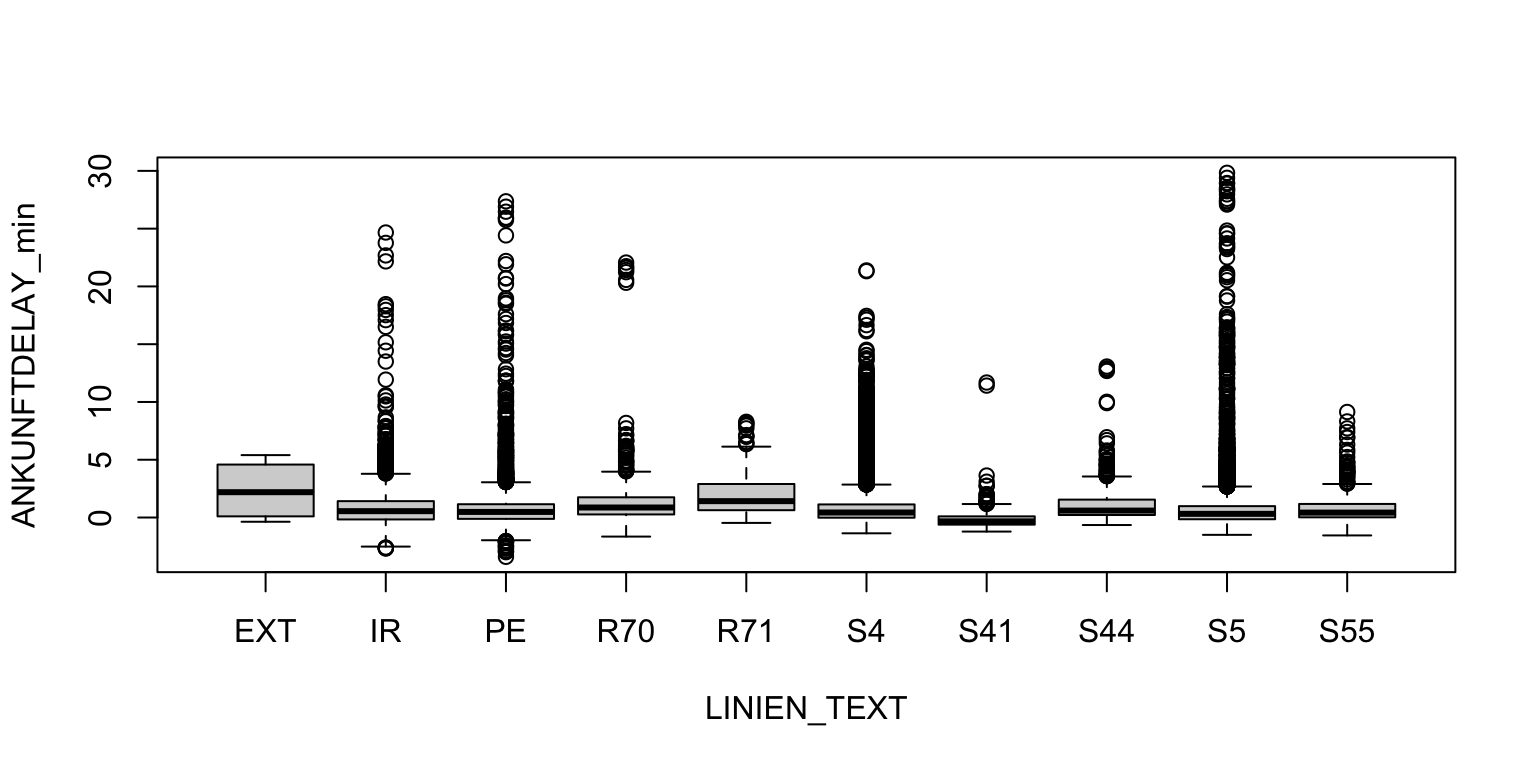
\includegraphics{final_documentation_files/figure-latex/boxplot-ANKUNFTDELAY_min-LINIEN_TEXT-1.pdf}

In the boxplot, we can see that the R71 has a relatively large variance
between the 25th and 75th percentiles of the data. Nevertheless, R71 has
fewer outliers compared to the other lines. The delays on R71 might be
consistent but not extreme enough to be detected as a significant
predictor in the GLM.

Although R71 has a relatively high average delay, this does not
necessarily imply that the line itself is a major factor in predicting
delays. The GLM is trying to predict the probability of a delay (yes/no)
based on various predictors. Other variables---such as weather, time of
day, or operational factors---might influence whether a delay occurs for
R71 trains.

Lets have now a look at the coefficients of glm\_delay

\begin{verbatim}
   (Intercept)  LINIEN_TEXTIR  LINIEN_TEXTPE LINIEN_TEXTR70 LINIEN_TEXTR71 
          0.67           0.09           0.07           0.09           0.46 
 LINIEN_TEXTS4 LINIEN_TEXTS41 LINIEN_TEXTS44  LINIEN_TEXTS5 LINIEN_TEXTS55 
          0.09           0.01           0.16           0.05           0.08 
\end{verbatim}

To interpret the effect of different train lines on delay likelihood,
the logistic regression coefficients were exponentiated to obtain odds
ratios. Compared to the baseline (EXT), all other lines show
significantly lower odds of delay. For example, line IR has 91\% lower
odds of delay, S41 has 99\% lower odds, and lines PE, R70, and S5 also
show substantial reductions (93\%, 91\%, and 95\% lower odds,
respectively). This confirms that EXT is far more prone to delays than
the other lines.

As a next step, we simulate predictions using the GLM to estimate the
likelihood of train delays, and then compare these simulated results
with the actual dataset.

\begin{verbatim}
 LINIEN_TEXT        predicted_prob    
 Length:10000       Min.   :0.008065  
 Class :character   1st Qu.:0.045756  
 Mode  :character   Median :0.054980  
                    Mean   :0.104591  
                    3rd Qu.:0.097059  
                    Max.   :0.400000  
\end{verbatim}

The mean of the simulated data is 0.105. This is the reason why we
cannot take a threshold of 0.5. This would result in nearly all cases
being classified as non-delayed, since very few predicted probabilities
exceed 0.5---ultimately leading to extremely poor sensitivity and almost
no true positives.

Several thresholds were tested to determine the optimal cut-off point
for classifying delays based on the predicted probabilities. Thresholds
such as 0.03, 0.08, and 0.1 were evaluated, but they either led to a
very low specificity or poor sensitivity. A threshold of 0.2 appeared to
offer the most reasonable trade-off between correctly identifying
delayed trains (sensitivity) and avoiding false delay predictions
(specificity), making it the most balanced choice for this model.

\begin{verbatim}
Confusion Matrix and Statistics

          Reference
Prediction     0     1
         0 43493  2175
         1 11006   545
                                          
               Accuracy : 0.7696          
                 95% CI : (0.7662, 0.7731)
    No Information Rate : 0.9525          
    P-Value [Acc > NIR] : 1               
                                          
                  Kappa : -6e-04          
                                          
 Mcnemar's Test P-Value : <2e-16          
                                          
            Sensitivity : 0.79805         
            Specificity : 0.20037         
         Pos Pred Value : 0.95237         
         Neg Pred Value : 0.04718         
             Prevalence : 0.95246         
         Detection Rate : 0.76011         
   Detection Prevalence : 0.79813         
      Balanced Accuracy : 0.49921         
                                          
       'Positive' Class : 0               
                                          
\end{verbatim}

The model's accuracy is 76.96\%, which at first glance suggests decent
performance, but this metric is heavily influenced by the significant
imbalance between delayed and non-delayed trains in the dataset. Due to
the high punctuality of Swiss trains, the vast majority of observations
are non-delays, making accuracy a somewhat misleading indicator of model
effectiveness.

Sensitivity, which captures how well the model identifies actual delays,
is fairly high at 79.8\%, indicating that the model detects most delay
cases. However, specificity is low at 20.0\%, meaning it struggles to
correctly identify non-delayed trains, frequently labeling them as
delayed. The model's precision is high at 95.2\%, so when it predicts a
delay, it is usually right.

On the other hand, the negative predictive value is low at 4.7\%,
reflecting poor performance in correctly predicting trains that are on
time.

Balanced accuracy, which considers both sensitivity and specificity, is
49.9\% suggesting the model performs no better than random guessing when
it comes to balancing delay and non-delay predictions.

The binomial Generalized Linear Model (GLM) successfully identifies
line-specific vulnerabilities and the overall likelihood of train delays
on the Zentralbahn network. Despite strong precision in predicting
delays, the model struggles with accurately identifying non-delayed
trains, largely due to class imbalance. This analysis provides a
critical step towards understanding operational bottlenecks, but further
refinement is needed to address specificity limitations. Targeted
improvements, such as better class balancing and threshold optimization,
could enhance model reliability and support Zentralbahn's goal of
improving punctuality and service efficiency.

\section{Poisson Model}\label{poisson-model}

\subsection{Overview}\label{overview}

The goal of this model is to predict the number of delayed trains based
on several predictors. The number of delayed trains is aggregated to
``operating hour'' and ``operation day''. This means:

\begin{itemize}
\tightlist
\item
  there are in total 660 observations
\item
  there are 30 observatios per ``operating hour'' because the dataset
  contains the month november, which has 30 days.
\item
  there are 22 observations per ``operating day'' because there are in
  total 23 operating hours , and between 1am and 2am there is no
  operation
\end{itemize}

Since the response variable is a count-variable, we expect it to exhibit
right skewness and increasing variance as the count increases.

Plotting the data reveals that indeed the count-variable is
right-skewed.

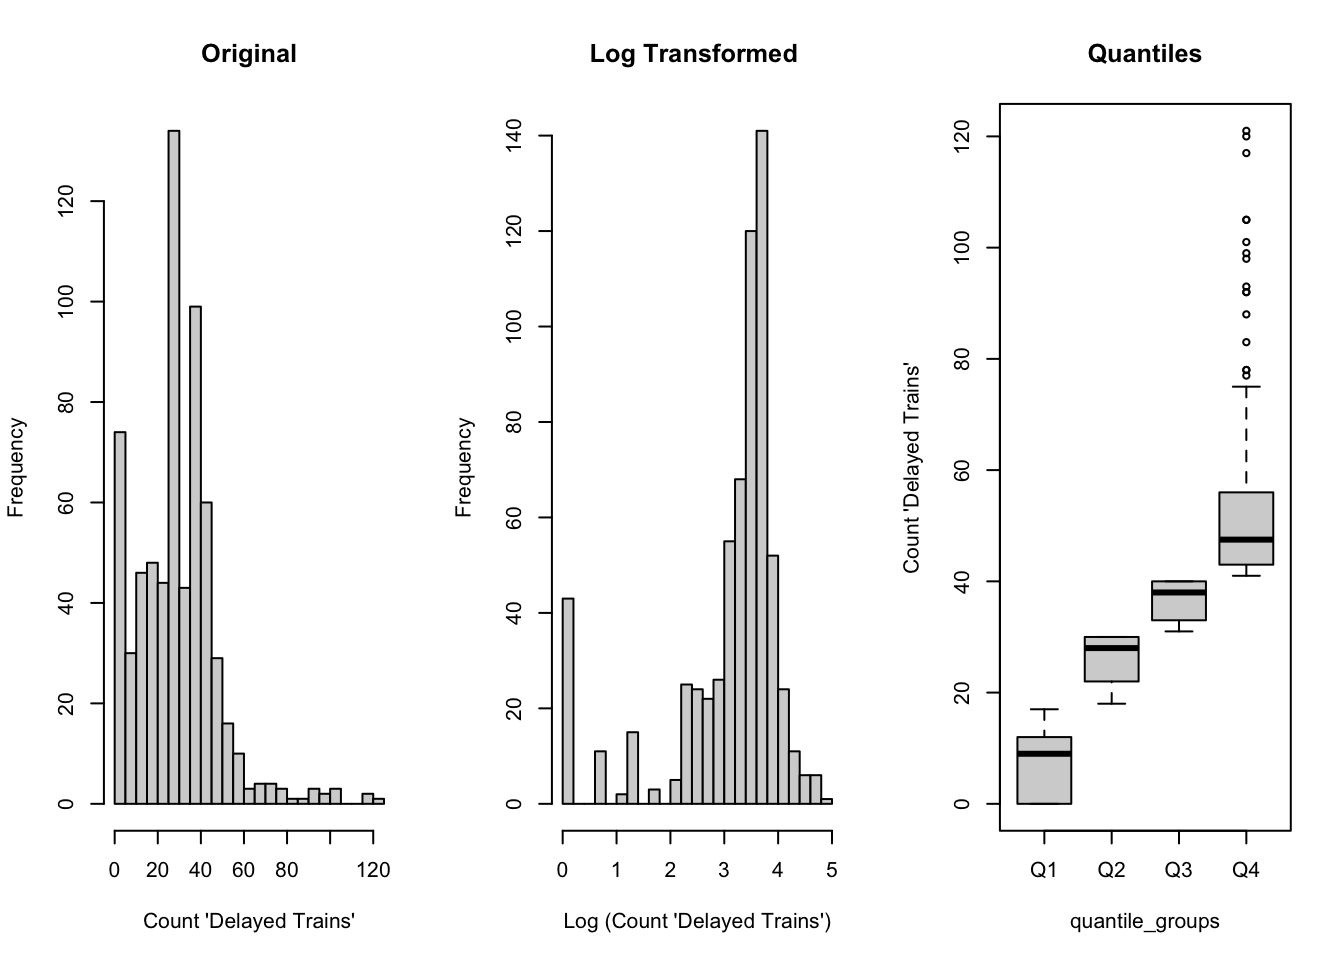
\includegraphics{final_documentation_files/figure-latex/Hist Skewed-1.pdf}

The quartile boxplot does not support the assumption that the variance
increases linearly with the mean. This suggests that the count variable
may not follow a Poisson distribution. This is an initial indication
that the GLM should be fitted with a quasipoisson family to account for
overdispersion.

\subsection{Finding reasonable
Predictors}\label{finding-reasonable-predictors}

\subsubsection{Operation Category''}\label{operation-category}

Having a predictor operating hour with 24 levels makes the
interpretation of the model quite complicated. Therefore a first
visualization of the data should give an idea if the predictor
``operating-hour'' can be simplified.

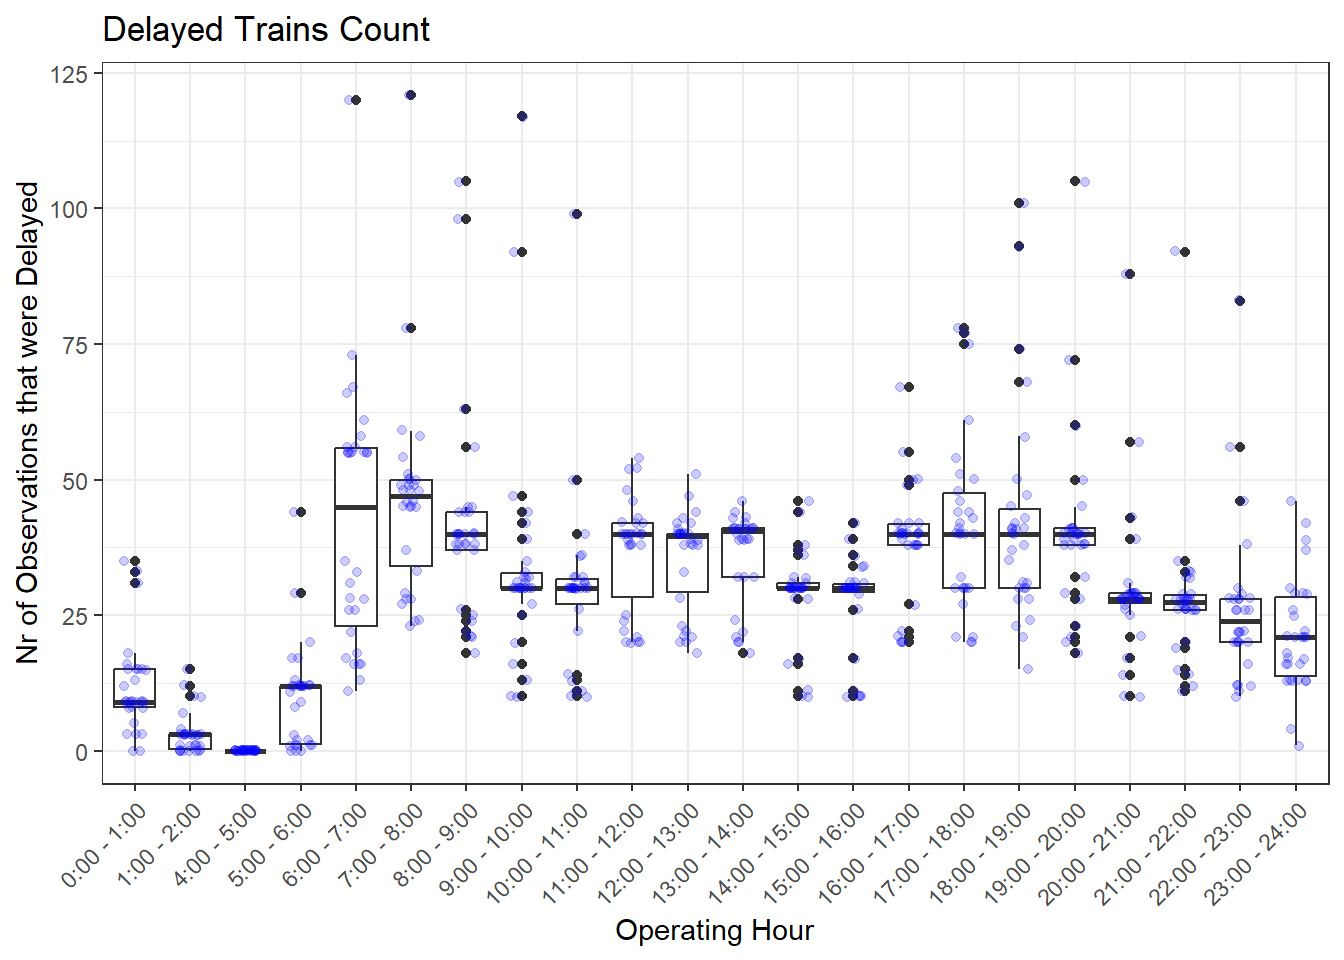
\includegraphics{final_documentation_files/figure-latex/Nr of Delay aggregated per Day and Operating Hour-1.pdf}

Indeed there seems to be a pattern in ``operation hour''. In a first
step, the ``operation- hour'' is simplified by ``operation category''
with 3 levels:

\begin{itemize}
\tightlist
\item
  Low Operation : (0:00 until 6:00)
\item
  Rush Hour : (6:00 until 9:00) and (11:00 until 14:00) and (16:00 until
  20:00)
\item
  Normal Operation : Everything else
\end{itemize}

The boxplot on the left compares the number of delayed trains across
operation categories, but this comparison is not meaningful because each
category has a different total number of train arrivals. On the right,
the delay counts are normalized by the total number of trains in each
category. As a result, the differences between the boxplots become less
pronounced but more interpretable

\begin{verbatim}
# A tibble: 3 x 2
  operation_category count
  <chr>              <int>
1 Low Operation       2841
2 Normal Operation   32718
3 Rush Hour          45515
\end{verbatim}

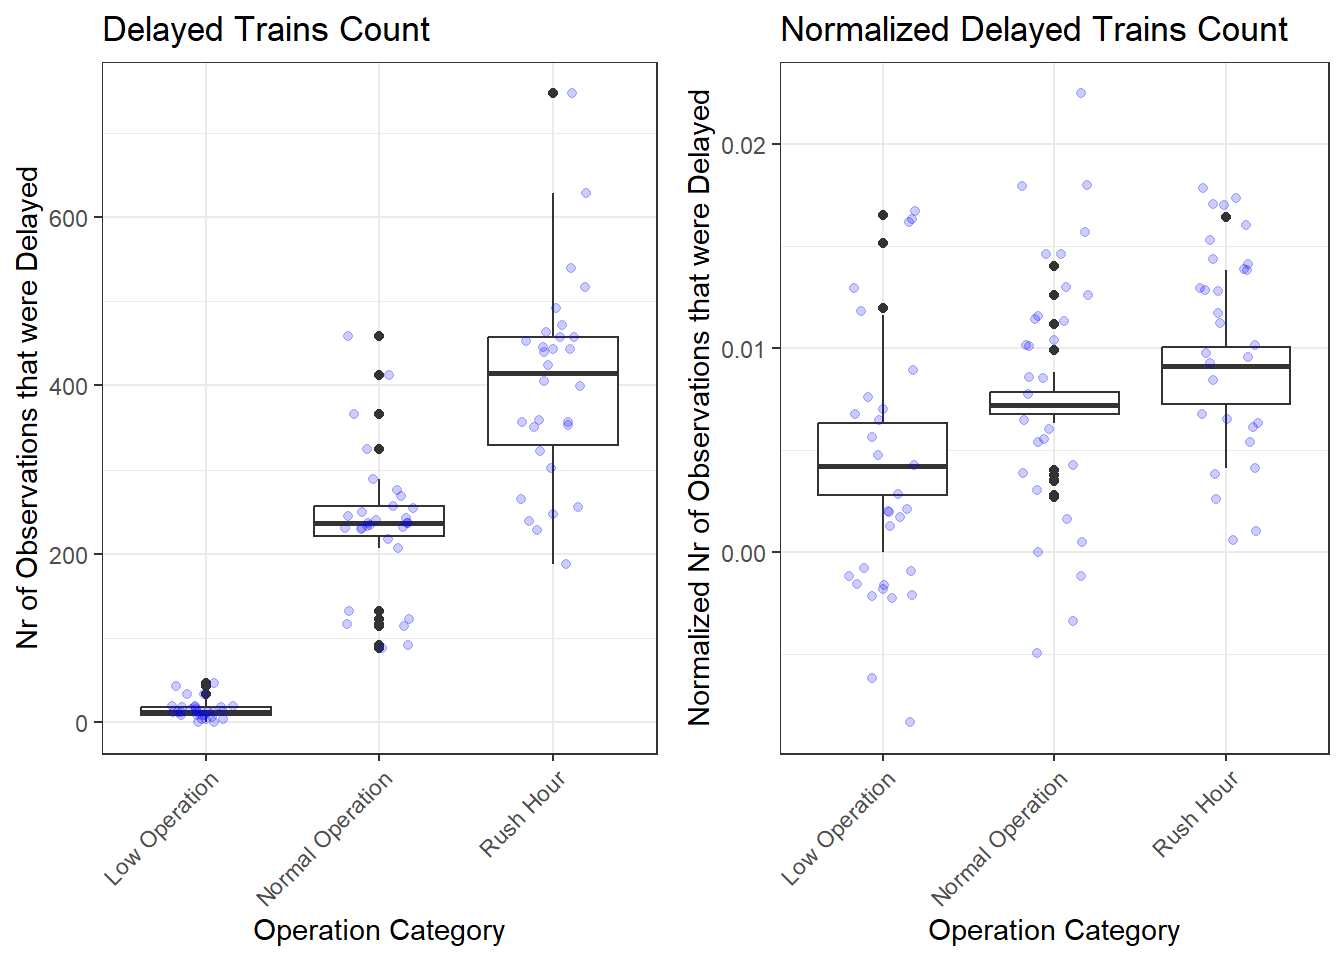
\includegraphics{final_documentation_files/figure-latex/Normalize for compariosn-1.pdf}

We now perform an ANOVA followed by multiple comparison testing to
statistically assess the differences observed in the normalized boxplot.

\begin{itemize}
\item
  ANOVA confirms that there is a statistically significant difference
  between at least one of the three operation categories.
\item
  The multiple comparison test reveals that not all pairwise differences
  are significant. While `Low Operation' differs significantly from both
  `Normal Operation' and `Rush Hour', the difference between `Normal
  Operation' and `Rush Hour' is not statistically significant.
\end{itemize}

This supports our earlier observation from the boxplot and confirms that
the predictor is overall significant, though not all categories differ
from each other

\begin{verbatim}
                   Df    Sum Sq   Mean Sq F value   Pr(>F)    
operation_category  2 0.0001913 9.566e-05   9.649 0.000164 ***
Residuals          87 0.0008625 9.910e-06                     
---
Signif. codes:  0 '***' 0.001 '**' 0.01 '*' 0.05 '.' 0.1 ' ' 1
\end{verbatim}

\begin{verbatim}

     Simultaneous Tests for General Linear Hypotheses

Multiple Comparisons of Means: Tukey Contrasts


Fit: aov(formula = Count_Delayed_Norm ~ operation_category, data = d.poisson.agg.day.oc)

Linear Hypotheses:
                                      Estimate Std. Error t value Pr(>|t|)    
Normal Operation - Low Operation == 0 0.001947   0.000813   2.394   0.0488 *  
Rush Hour - Low Operation == 0        0.003566   0.000813   4.387   <1e-04 ***
Rush Hour - Normal Operation == 0     0.001620   0.000813   1.992   0.1201    
---
Signif. codes:  0 '***' 0.001 '**' 0.01 '*' 0.05 '.' 0.1 ' ' 1
(Adjusted p values reported -- single-step method)
\end{verbatim}

To conclude, the analysis has revealed a valuable predictor that will be
utilized in the subsequent modeling phase

\subsubsection{``Event Category''}\label{event-category}

Creating a level for each Day in November does not make sense. Therefore
data are again visualized to see if there are any patterns so that
predictor can be simplified. In the boxplot there are 22 observation per
``operation day''. One obsevation per operating hour.

The boxplot proposes a separtion into the following 3 Levels:

\begin{itemize}
\tightlist
\item
  Extreme Days: 22.11 and 23.11
\item
  Meiringen Reopened : From 25.11 on(see more
  \href{https://www.zentralbahn.ch/de/kennenlernen/die-zentralbahn/einblicke/wiedereroeffnung-der-strecke-meiringen-interlaken-ost-am-25-november-2024\%7D}{here}
\item
  Normal Operation
\end{itemize}

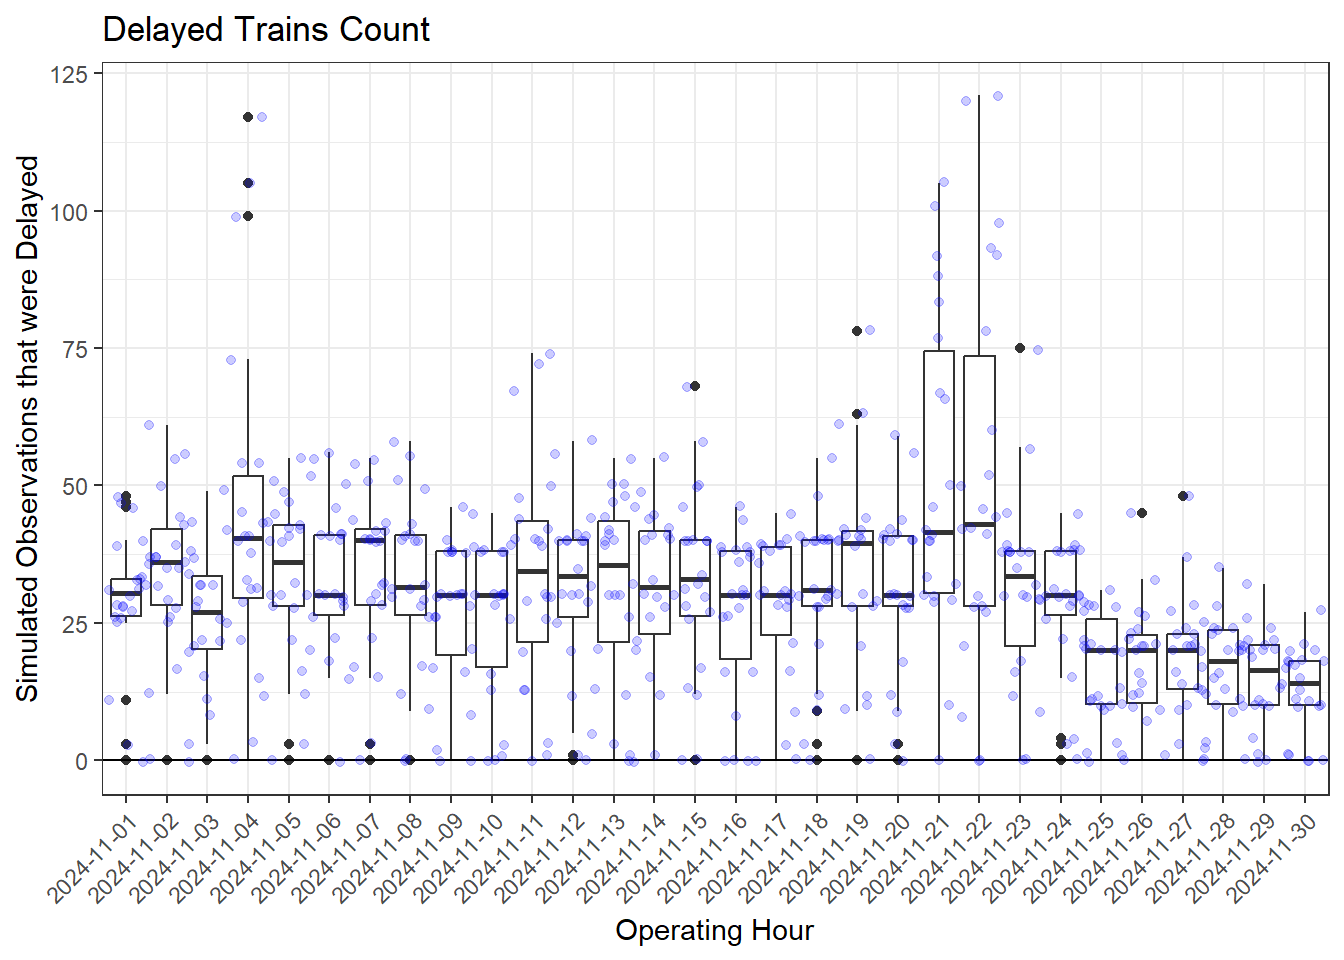
\includegraphics{final_documentation_files/figure-latex/Look at Days-1.pdf}

The boxplot on the left compares the number of delayed trains across
event categories, but this comparison is not meaningful because each
category has a different total number of train arrivals. On the right,
the delay counts are normalized by the total number of trains in each
category. As a result, the differences between the boxplots become less
pronounced but more interpretable

\begin{verbatim}
# A tibble: 3 x 2
  event_category     count
  <chr>              <int>
1 Extreme Days        5515
2 Meiringen Reopened 16323
3 Normal Operation   59236
\end{verbatim}

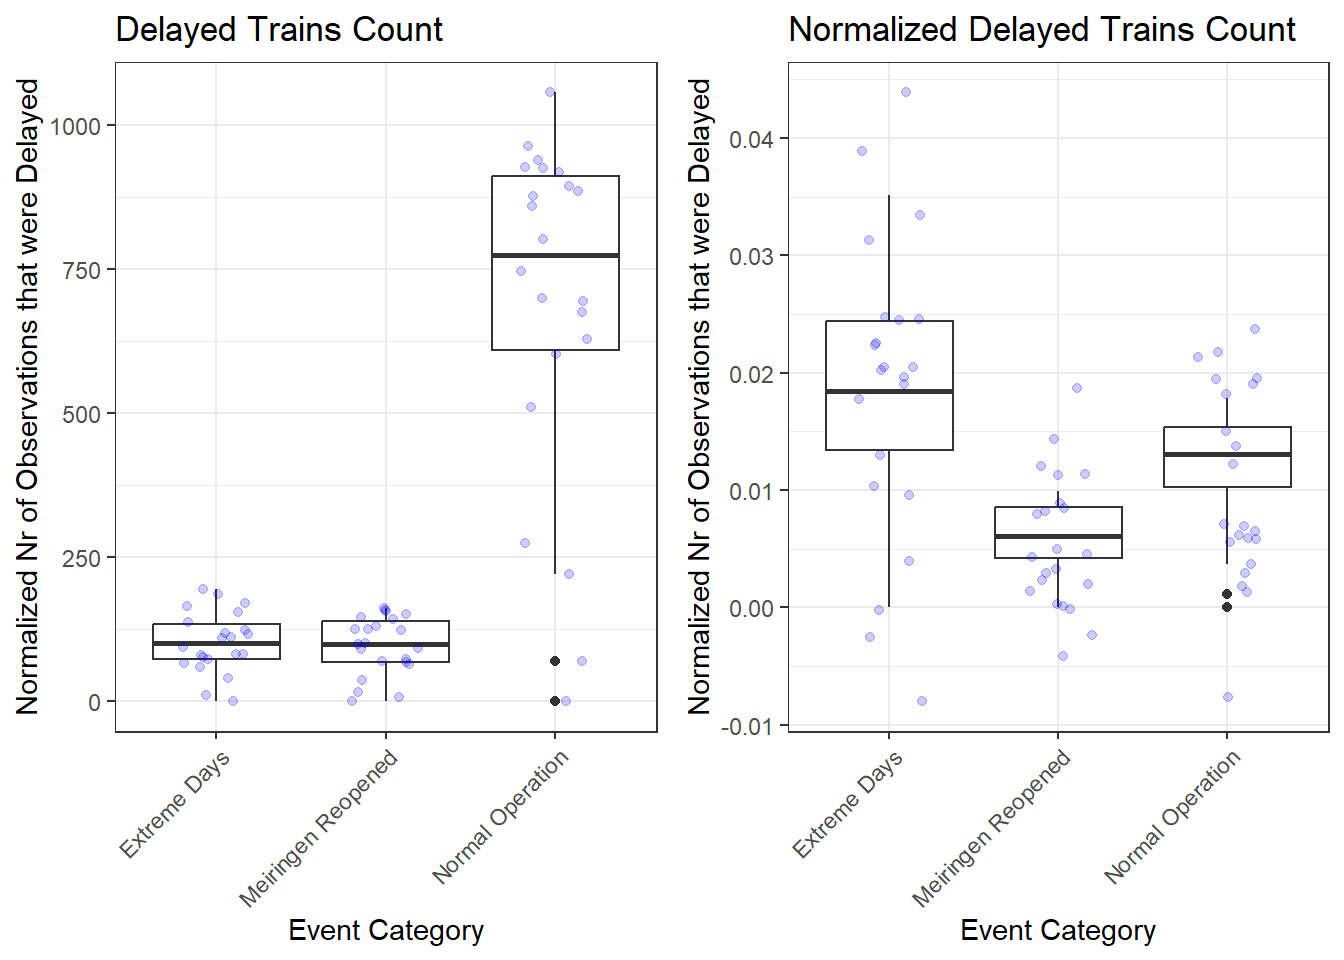
\includegraphics{final_documentation_files/figure-latex/Normalize for comparison 2-1.pdf}

To statistically assess the differences observed in the boxplot, we
conduct an ANOVA followed by multiple comparison testing.

\begin{itemize}
\item
  The ANOVA confirms that there is a statistically significant
  difference between at least one of the three day categories.
\item
  The multiple comparison test further reveals that all pairwise
  differences between the categories are statistically significant.
\end{itemize}

This indicates that event\_category is a strong predictor and will be
considered for inclusion in the modeling process.

\begin{verbatim}
               Df   Sum Sq   Mean Sq F value   Pr(>F)    
event_category  2 0.001753 0.0008766   20.86 1.12e-07 ***
Residuals      63 0.002647 0.0000420                     
---
Signif. codes:  0 '***' 0.001 '**' 0.01 '*' 0.05 '.' 0.1 ' ' 1
\end{verbatim}

\begin{verbatim}

     Simultaneous Tests for General Linear Hypotheses

Multiple Comparisons of Means: Tukey Contrasts


Fit: aov(formula = Count_Delayed_Norm ~ event_category, data = d.poisson.agg.day.dc)

Linear Hypotheses:
                                            Estimate Std. Error t value
Meiringen Reopened - Extreme Days == 0     -0.012604   0.001954  -6.449
Normal Operation - Extreme Days == 0       -0.006917   0.001954  -3.539
Normal Operation - Meiringen Reopened == 0  0.005687   0.001954   2.910
                                           Pr(>|t|)    
Meiringen Reopened - Extreme Days == 0      < 1e-04 ***
Normal Operation - Extreme Days == 0        0.00213 ** 
Normal Operation - Meiringen Reopened == 0  0.01359 *  
---
Signif. codes:  0 '***' 0.001 '**' 0.01 '*' 0.05 '.' 0.1 ' ' 1
(Adjusted p values reported -- single-step method)
\end{verbatim}

\subsubsection{Temperature and
Precipitation}\label{temperature-and-precipitation}

Weather data may also influence train delays. In the dataset, daily
weather variables such as precipitation and temperature are available
for the Lucerne region. However, initial visualizations do not reveal
any clear correlation between weather conditions and the number of
delayed trains. Despite this, the weather variables are still included
in the GLM to assess whether they contribute any predictive value that
is not immediately apparent from the visual analysis.

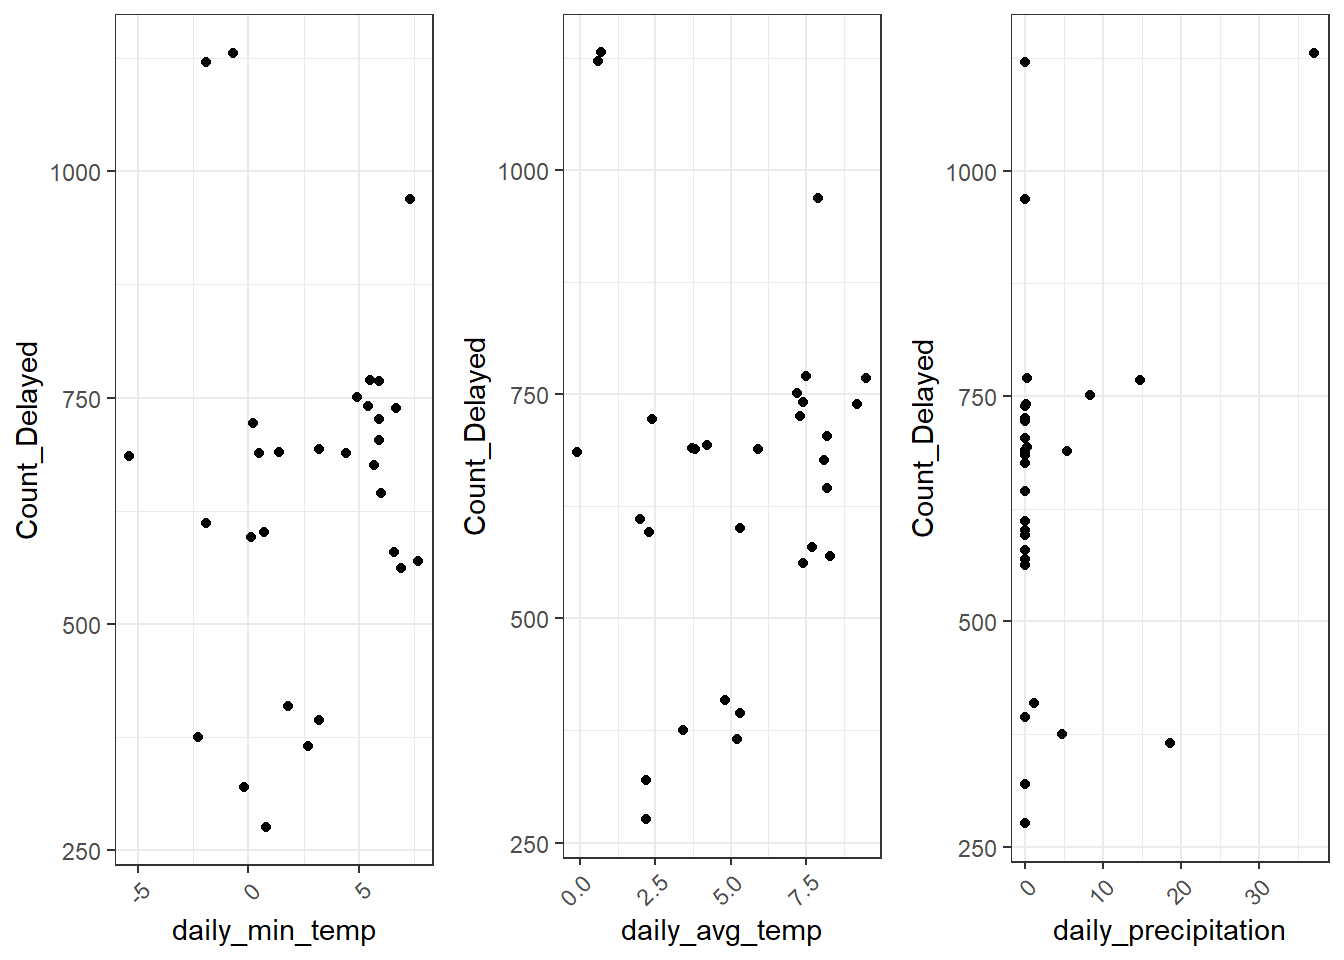
\includegraphics{final_documentation_files/figure-latex/Weather Data-1.pdf}

\subsection{Building the GLM model}\label{building-the-glm-model}

``Prior to building the model, 80\% of the available data was randomly
selected for training. For simplicity, the training data was chosen
without stratification.

To simplify model interpretation, the reference level for both Event
Category and Operation Category was set to ``Normal operation''. This
choice facilitates clearer comparisons and makes the interpretation of
model coefficients more intuitive.

\begin{Shaded}
\begin{Highlighting}[]
\CommentTok{\# Prepare Reference Level to Normal Operation}
\NormalTok{trainData}\SpecialCharTok{$}\NormalTok{event\_category }\OtherTok{\textless{}{-}} \FunctionTok{as.factor}\NormalTok{(trainData}\SpecialCharTok{$}\NormalTok{event\_category) }\SpecialCharTok{\%\textgreater{}\%} 
  \FunctionTok{relevel}\NormalTok{(}\AttributeTok{ref =} \StringTok{"Normal Operation"}\NormalTok{)}
\NormalTok{trainData}\SpecialCharTok{$}\NormalTok{operation\_category }\OtherTok{\textless{}{-}} \FunctionTok{as.factor}\NormalTok{(trainData}\SpecialCharTok{$}\NormalTok{operation\_category) }\SpecialCharTok{\%\textgreater{}\%} 
  \FunctionTok{relevel}\NormalTok{(}\AttributeTok{ref =} \StringTok{"Normal Operation"}\NormalTok{)}
\end{Highlighting}
\end{Shaded}

The initial GLM includes the promising predictors: Operation Category
and Event Category. Additionally, it also includes weather-related
predictors, which, though not particularly promising, are included to
explore their impact. These include Daily Min. Temperature, which is
more relevant than the average temperature as extreme temperatures may
cause technical defects, and Daily Precipitation.

Looking at the summary, it becomes clear that the weather data do not
significantly contribute to the model.

\emph{Note}: The GLM was run with the ``quasipoisson'' family due to
overdispersion. If the model were run with the ``poisson'' family, the
predictor ``daily\_min\_temp'' and ``daily\_precipitation'' would appear
significant, which is clearly incorrect.

\begin{Shaded}
\begin{Highlighting}[]
\NormalTok{glm }\OtherTok{\textless{}{-}} \FunctionTok{glm}\NormalTok{(Count\_Delayed }\SpecialCharTok{\textasciitilde{}}\NormalTok{ operation\_category }\SpecialCharTok{+}\NormalTok{ event\_category }\SpecialCharTok{+}\NormalTok{ daily\_min\_temp }\SpecialCharTok{+}\NormalTok{ daily\_precipitation,}
\AttributeTok{family =} \StringTok{"quasipoisson"}\NormalTok{, }\AttributeTok{data =}\NormalTok{ trainData)}

\FunctionTok{summary}\NormalTok{(glm)}
\end{Highlighting}
\end{Shaded}

\begin{verbatim}

Call:
glm(formula = Count_Delayed ~ operation_category + event_category + 
    daily_min_temp + daily_precipitation, family = "quasipoisson", 
    data = trainData)

Coefficients:
                                  Estimate Std. Error t value Pr(>|t|)    
(Intercept)                       3.267562   0.038505  84.860  < 2e-16 ***
operation_categoryLow Operation  -1.635018   0.118009 -13.855  < 2e-16 ***
operation_categoryRush Hour       0.435519   0.035864  12.144  < 2e-16 ***
event_categoryExtreme Days        0.513851   0.077597   6.622 8.83e-11 ***
event_categoryMeiringen Reopened -0.659573   0.059305 -11.122  < 2e-16 ***
daily_min_temp                    0.011188   0.006005   1.863    0.063 .  
daily_precipitation               0.002738   0.002362   1.159    0.247    
---
Signif. codes:  0 '***' 0.001 '**' 0.01 '*' 0.05 '.' 0.1 ' ' 1

(Dispersion parameter for quasipoisson family taken to be 4.559697)

    Null deviance: 6887.5  on 527  degrees of freedom
Residual deviance: 2388.5  on 521  degrees of freedom
AIC: NA

Number of Fisher Scoring iterations: 6
\end{verbatim}

What is evident from the summary is also confirmed by the Drop 1
analysis:

\begin{itemize}
\item
  Operation Category significantly increases the deviance, indicating
  its importance as a predictor.
\item
  The same applies to Event Category, which also contributes
  meaningfully to the model.
\item
  In contrast, the weather data does not appear to be useful predictors,
  as removing them does not substantially affect the deviance.
\end{itemize}

\begin{Shaded}
\begin{Highlighting}[]
\FunctionTok{drop1}\NormalTok{(glm, }\AttributeTok{Test =} \StringTok{"F"}\NormalTok{)}
\end{Highlighting}
\end{Shaded}

\begin{verbatim}
Single term deletions

Model:
Count_Delayed ~ operation_category + event_category + daily_min_temp + 
    daily_precipitation
                    Df Deviance
<none>                   2388.5
operation_category   2   5436.8
event_category       2   3537.6
daily_min_temp       1   2404.5
daily_precipitation  1   2394.6
\end{verbatim}

\emph{Therefore for the final model the weather data is dropped!}

\begin{Shaded}
\begin{Highlighting}[]
\NormalTok{glm }\OtherTok{\textless{}{-}} \FunctionTok{glm}\NormalTok{(Count\_Delayed }\SpecialCharTok{\textasciitilde{}}\NormalTok{ operation\_category }\SpecialCharTok{+}\NormalTok{ event\_category,}
\AttributeTok{family =} \StringTok{"quasipoisson"}\NormalTok{, }\AttributeTok{data =}\NormalTok{ trainData)}
\end{Highlighting}
\end{Shaded}

\begin{Shaded}
\begin{Highlighting}[]
\NormalTok{glm }\OtherTok{\textless{}{-}} \FunctionTok{glm}\NormalTok{(Count\_Delayed }\SpecialCharTok{\textasciitilde{}}\NormalTok{ operation\_category }\SpecialCharTok{+}\NormalTok{ event\_category,}
\AttributeTok{family =} \StringTok{"quasipoisson"}\NormalTok{, }\AttributeTok{data =}\NormalTok{ trainData)}

\FunctionTok{summary}\NormalTok{(glm)}
\end{Highlighting}
\end{Shaded}

\begin{verbatim}

Call:
glm(formula = Count_Delayed ~ operation_category + event_category, 
    family = "quasipoisson", data = trainData)

Coefficients:
                                 Estimate Std. Error t value Pr(>|t|)    
(Intercept)                       3.31586    0.03020 109.803   <2e-16 ***
operation_categoryLow Operation  -1.63259    0.11870 -13.753   <2e-16 ***
operation_categoryRush Hour       0.43698    0.03608  12.110   <2e-16 ***
event_categoryExtreme Days        0.49912    0.05590   8.928   <2e-16 ***
event_categoryMeiringen Reopened -0.68605    0.05631 -12.184   <2e-16 ***
---
Signif. codes:  0 '***' 0.001 '**' 0.01 '*' 0.05 '.' 0.1 ' ' 1

(Dispersion parameter for quasipoisson family taken to be 4.617011)

    Null deviance: 6887.5  on 527  degrees of freedom
Residual deviance: 2412.9  on 523  degrees of freedom
AIC: NA

Number of Fisher Scoring iterations: 6
\end{verbatim}

\begin{Shaded}
\begin{Highlighting}[]
\FunctionTok{exp}\NormalTok{(}\FunctionTok{coef}\NormalTok{(glm))}
\end{Highlighting}
\end{Shaded}

\begin{verbatim}
                     (Intercept)  operation_categoryLow Operation 
                      27.5461579                        0.1954231 
     operation_categoryRush Hour       event_categoryExtreme Days 
                       1.5480177                        1.6472706 
event_categoryMeiringen Reopened 
                       0.5035634 
\end{verbatim}

\subsection{Results}\label{results-1}

The model provides the following results:

\begin{itemize}
\item
  Intercept: On a normal operation day and during normal operation
  hours, the average number of delayed observations is 28 per hour.
\item
  Changing the operation to ``Low Operation'' (while keeping all other
  factors constant) results in an average of 28 * 0.2 ≈ 6 delayed
  observations per hour.
\item
  Changing the operation to ``Rush Hour'' (while keeping all other
  factors constant) results in an average of 28 * 1.5 = 42 delayed
  observations per hour.
\item
  Changing the event to ``Extreme Days'' (while keeping all other
  factors constant) results in an average of 28 * 1.6 = 45 delayed
  observations per hour.
\item
  Changing the event to ``Meiringen Reopened'' (while keeping all other
  factors constant) results in an average of 28 * 0.5 = 14 delayed
  observations per hour.
\end{itemize}

\subsection{Validation}\label{validation}

The remaining 132 observations were used to evaluate the model's
performance. The plot below highlights considerable uncertainty in the
predictions, especially for larger count values, where the model tends
to significantly underestimate the actual counts. This may be attributed
to the limited number of delay instances in the dataset.
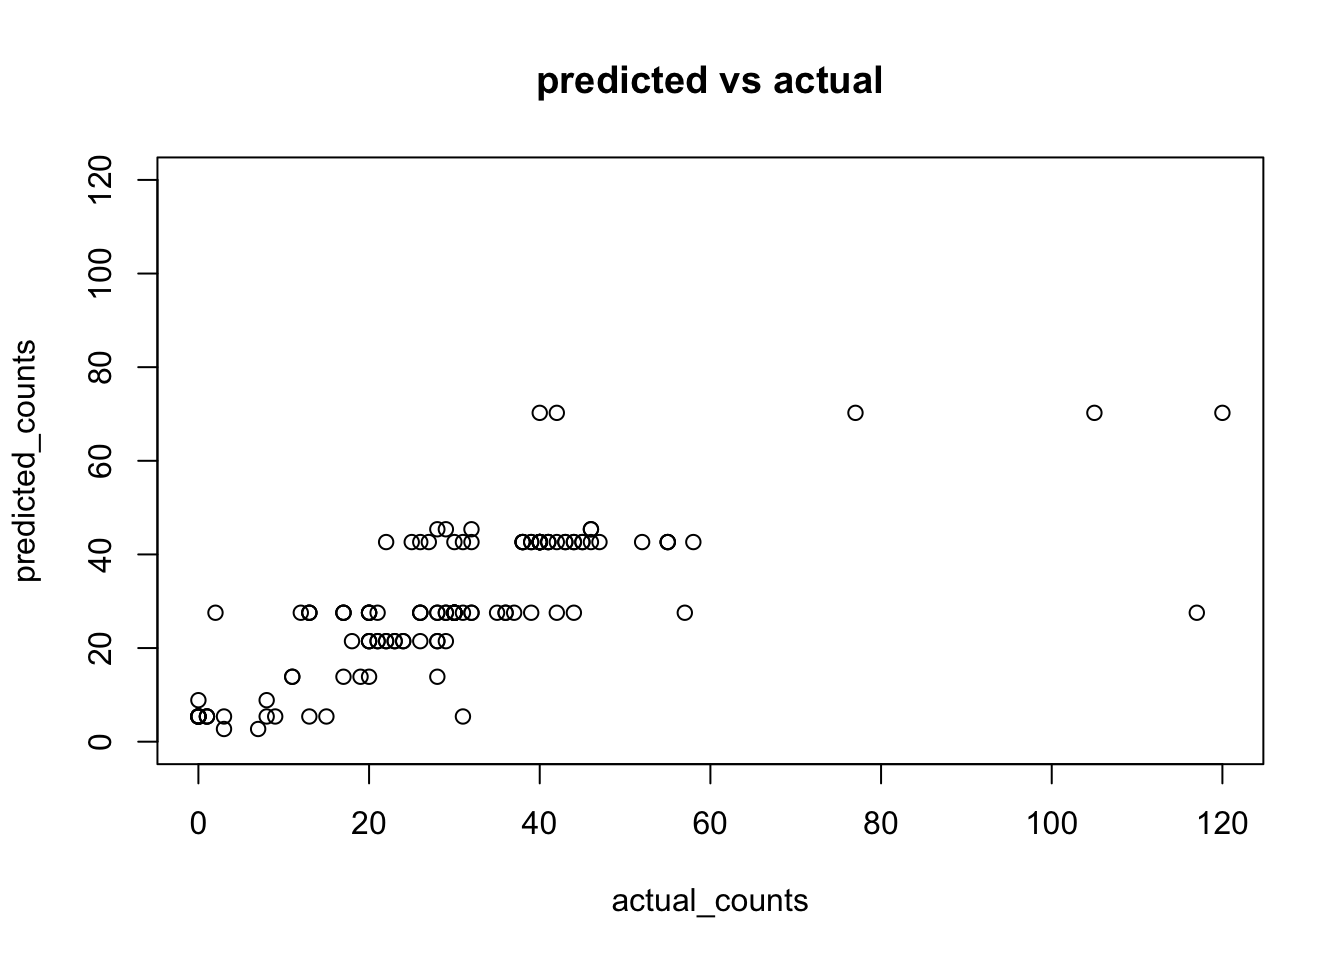
\includegraphics{final_documentation_files/figure-latex/Model Validation-1.pdf}

\subsection{Conclusion}\label{conclusion}

The model allows for rough predicting the expected number of delayed
trains per hour across different event and operational categories.
However, it's important to keep in mind that the number of delayed
trains per category is correlated with the total number of trains
operating during that category. Naturally, the more trains are in
operation, the higher the likelihood of delays.

\section{Use of Generative AI}\label{use-of-generative-ai}

ChatGPT can be a valuable tool for various aspects of programming,
particularly for detecting syntax errors and generating initial plots
quickly. It provides immediate feedback, making it easier for users to
identify issues and visually present their data. This speed and
convenience can help jump-start the coding process, especially for
beginners or when exploring new concepts.

However, there are limitations to relying solely on ChatGPT for more
complex tasks. While it can help create basic plots, developing more
specific or tailored visualizations often leads users down a ``rabbit
hole,'' where time is spent refining the plot rather than focusing on
the underlying analysis. Additionally, implementing modularity in code
is challenging when using ChatGPT. It requires a deeper understanding of
programming concepts to ensure code is reusable, maintainable, and
efficient, which cannot always be achieved through AI-generated
solutions alone.

Another significant concern is that the code generated by ChatGPT is
often done quickly, but it may lack proper documentation and clarity.
Without adequate comments and explanations, the code can be difficult to
read and understand, posing challenges for collaboration or future
revisions. Furthermore, ChatGPT sometimes generates overly complex
solutions when a simpler, more efficient approach could be used, which
could be easily implemented with just a few lines of code if the
programmer has a solid grasp of the task at hand.

As data scientists, it is essential not only to understand the technical
aspects of coding but also to gain a deep understanding of the data
itself. Data analysis is a creative process that involves continuous
iteration, exploration, and insight. To arrive at meaningful
conclusions, data scientists must engage with domain experts and other
stakeholders throughout the analysis process. This collaboration helps
ensure that the results are accurate, relevant, and actionable,
ultimately leading to well-informed decisions.

In conclusion, while ChatGPT offers valuable assistance in coding,
especially for quick debugging and basic tasks, it is important for
users to ensure they understand their code thoroughly and the data they
are working with. Achieving effective modularity, clarity, and
efficiency requires a combination of technical expertise and creativity,
with ongoing collaboration, to ensure the success of data analysis
projects

\section{Conclusion}\label{conclusion-1}

The analysis confirmed what Zentralbahn had likely anticipated: a
\textbf{severe thunderstorm} caused substantial disruption to train
operations, as documented in the official report on the reopening of the
\textbf{Meiringen--Interlaken Ost} route on \textbf{November 25,
2024}(\href{https://www.zentralbahn.ch/de/kennenlernen/die-zentralbahn/einblicke/wiedereroeffnung-der-strecke-meiringen-interlaken-ost-am-25-november-2024}{source}).

In addition to this expected finding, several other valuable insights
were uncovered through the application of various statistical models.
Importantly, \textbf{the models developed can be used to predict delays
under different operational conditions}, providing a foundation for
proactive planning and decision-making.

\textbf{1. High Delay Probability for ``EXT'' Trains}

Extra trains (``EXT'') were found to have the highest probability of
delay. A likely reason is the use of older trainsets, which may be less
reliable or slower to adapt to schedule changes.\\
The model allows for \textbf{predicting the likelihood of delay} for
individual train entries based on their train type and other features,
enabling early intervention or scheduling adjustments.

\textbf{2. Limited Influence of Weather}

Weather conditions showed only a \textbf{limited direct effect} on train
delays. This is likely due to \textbf{low temporal resolution} in the
available weather data.\\
Still, the model can be used to \textbf{quantify expected delay
contributions from weather} where data is available, and it is ready to
be improved once finer-grained weather data is incorporated.

\textbf{3. Operational Patterns and Delay Clusters}

The model identified three distinct operational time categories, with
\textbf{rush hours} exhibiting the most frequent delays. While traffic
volume is a plausible factor, this recurring pattern hints at
\textbf{systemic scheduling or resource constraints}.\\
With this model, it is possible to \textbf{predict the expected number
of delays per hour} based on operational time and other variables,
supporting staffing and dispatch decisions.

Defined operational periods:

\begin{itemize}
\tightlist
\item
  \textbf{Low Operation:} 00:00 -- 06:00\\
\item
  \textbf{Rush Hour:} 06:00 -- 09:00, 11:00 -- 14:00, and 16:00 --
  20:00\\
\item
  \textbf{Normal Operation:} All other times
\end{itemize}

\textbf{4. Noteworthy Dates and Events}

The following dates and events stood out in the analysis and can inform
the refinement of future models:

\begin{itemize}
\tightlist
\item
  \textbf{Extreme Delay Days:} November 22 and 23, 2024 -- identified as
  outlier days with unusually high delays\\
\item
  \textbf{Route Reopening:} From \textbf{November 25, 2024}, the
  Meiringen--Interlaken Ost line resumed normal service
  (\href{https://www.zentralbahn.ch/de/kennenlernen/die-zentralbahn/einblicke/wiedereroeffnung-der-strecke-meiringen-interlaken-ost-am-25-november-2024}{details})\\
\item
  \textbf{Return to Normal Operation:} Delay patterns normalized after
  the disruption, serving as a \textbf{benchmark period for predictive
  model calibration}
\end{itemize}

\end{document}
